\documentclass[twocolumn,11pt,english]{article}
\usepackage{comment}
\usepackage{tikz}
\usepackage{graphicx}
\usepackage{wrapfig}
\usepackage{cite}
\usepackage{relsize}
\usepackage[T1]{fontenc}
\usepackage[margin=1.0in]{geometry}
\usepackage{pstricks}
\usepackage{pgfplots}

\title{Blowship - Untraceable Low-Latency Message Transfer via a Central Server}
\date{}
\author{
  Carlyle, John\\
  \textit{jcarlyle@ucsc.edu}
  \and
  McDermott, Morgan\\
  \textit{moamcder@ucsc.edu}
}

\begin{document}
\maketitle

\section*{Abstract} 
Many systems have been developed that preserve the anonymity of the sender and receiver of data. These systems are typically decentralized, routing messages through some series of trusted or untrusted peers and servers. 

In this paper we present a centralized anonymity system that uses a single, untrusted central server, adapting decentralized peer-to-peer (P2P) protocols to work in this context, and combine these with Computational Private Information Retrieval (CPIR) to enable low-latency, low-overhead anonymous communication. The primary reason behind a central server is to have a browser based service which needs a server to route for a pseudo-P2P network.

\section{Introduction}

Traditional cryptography hides the message being sent from one party to another. This is useful for many purposes, but there is an important aspect of your communication that is freely availble to anyone observing the transfer: the connection between sender and recipient. 

Much work has been done to build networks that can obscure this connection by passing the message through a series of peers in such a way that no peer, or even large group of peers, can determine its destination. Many of these systems route the message through dedicated peers that are always online (as with Mix systems \cite{chaum-mix}, like the popular Tor\cite{tor-design} anonymity system). Many of these systems are designed to relay email and as such have high latency (as in \cite{minion-design}, although there are systems like Tor designed specifically to have low latency. 

In most cases, these systems are highly decentralized. In Tor for example, the relay servers used are chosen by the client \cite{tor-design}, and the only ``central authority'' are the trusted directory servers. In this paper we explore building a highly centralized system, for use in cases where decentralization is difficult and to explore possible benefits. 

Current browsers have limited P2P communication capability - currently, they only have the ability to facilitate P2P distribution of media like video \cite{daoust2012towards}, and can't communicate with general purpose messages. For this reason, there are no pure P2P anonymization networks that operate at the browser level without using plugins. 

We present to the reader Untraceable Low-Latency Messaging via a Central Server. Our message system is accessed via the browser, allowing a person to browse to one central location and conveniently use this service, rather than using an external program for anonymity as with existing P2P services. The central server acts as an intermediary and facilitator for the network of peers using it. The peers are used to obsfucate who is sending messages to whom, allowing the clients to maintain anonymity and message security, in as close to real time as possible.

\section{Previous Work}
The majority of research into anonymous communication uses decentralized P2P networks. In our work, we develop a centralized anonymous communication network using principles and protocols from these decentralized systems. 

\subsection{Mixes}
Mixes are servers through which encrypted messages are sent, hiding the correlation between incoming and outgoing messages using encryption, pooling incoming messages, and a variety of other strategies\cite{chaum-mix}. Mixes have seen wide use since Chaum first introduced them in 1981 \cite{chaum-mix}. In his protocol, mixes encrypt messages using public-private key cryptography so that incoming and outgoing messages have different content. For further security, messages have a fixed size, and mixes reorder messages before relaying them. 

 Mixes have been used in systems such as MixMinion\cite{minion-design} to anonymously send and receive email. Onion routing systems such as Tor \cite{tor-design} use a series of mixes as proxies for data. 

Some systems use a fixed route of Mixes (as in MixMinion), while others allow clients to choose their own route through the mixes (as in Tor).

The anonymity mixes provide depends on many factors and was thoroughly analyzed by Serjantov~\cite{trickle02}. In our system we use peers in the network as mixes, and will analyze their security using the known attacks that Serjantov presents (See Section~\ref{sec:PeersAsMixes} for a more in depth discussion). 

\subsection{Nym systems} Pseudonymous message delivery systems enable users to send and receive messages with a \textit{nym} (pseudonym) that cannot be traced back to their true identity \cite{sassaman:wpes2005}. Many of these systems rely on having an anonymous ``forward'' channel that allows a user to send a message without attackers being able to deduce the recipient. Our paper implements exactly this forward channel, and so could easily be coupled with a Nym system. 

\subsection{Private Information Retrieval} 

Private Information Retrieval, first introduced by Chor and Goldreich \cite{pir}, allows a user to access information from a database without the database server learning the user's query. 

The trivial way of achieving this is to send the user the entire database. Although this is actually used in systems like Tor\cite{tor-design}, it may not be practical given a database with thousands or possibly millions of records.

The first Private Information Retrieval databases developed were  Information-Theoretical PIR (ITPIR), and operate by separating data between multiple servers\cite{pir}. This model is fairly efficient, although it assumes the servers won't collude to discover user queries. 

It was discovered that PIR is possible with a single server. Computational PIR (first introduced by Chor \cite{CPIR}) uses computationally difficult mechanisms to prevent a server hosting a single database from learning which records users retrieve from it. 

In all known PIR systems, query anonymity comes at a cost. It has been shown that the database must perform an $O(n)$ operation to respond to each query\cite{CPIR}, where $n$ is the size of the database. If this weren't the case, the database wouldn't touch every bit in the database to respond to a query and would gain some information about the query itself. 

Additionally, there is communication overhead in all known PIR systems. Responses to queries are usually polynomial or polylogarithmic in $n$ \cite{CPIR} \cite{pir}. 

Private Information Retrieval has been used to facilitate anonymous communication in a variety of ways. The Pynchon Gate \cite{sassaman:wpes2005} is a nym system that uses information-theoretic PIR as a layer of indirection between a user and their nym - allowing users to retrieve mail sent to their nym with information-theoretic privacy guarantees. Tor-PIR \cite{MittalOTBG11} uses PIR to distribute information about servers without forcing users to download the entire directory. In our paper, we use PIR for directory services and investigate the possibility of using it for anonymous communication. 

\section{Conventions}
All logs in this paper are $\log_2$ unless otherwise specified. $N$ is the total number of peers in the network. A \textit{hop} is defined as a message passing from $peer_a$ to the server and then to $peer_b$, for reasons explained in section 5.
\begin{figure}[ht]
  \begin{center}
    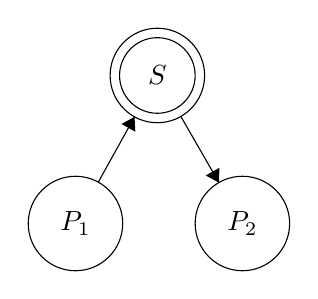
\begin{tikzpicture}[scale=0.2]
      \tikzstyle{every node}+=[inner sep=0pt]
      \draw [black] (32.9,-14.9) circle (3);
      \draw (32.9,-14.9) node {$S$};
      \draw [black] (32.9,-14.9) circle (2.4);
      \draw [black] (27.7,-24.3) circle (3);
      \draw (27.7,-24.3) node {$P_1$};
      \draw [black] (38.3,-24.3) circle (3);
      \draw (38.3,-24.3) node {$P_2$};
      \draw [black] (29.15,-21.67) -- (31.45,-17.53);
      \fill [black] (31.45,-17.53) -- (30.62,-17.98) -- (31.5,-18.47);
      \draw [black] (34.39,-17.5) -- (36.81,-21.7);
      \fill [black] (36.81,-21.7) -- (36.84,-20.76) -- (35.97,-21.25);
    \end{tikzpicture}
  \end{center}
\caption{A hop between two peers}
\end{figure}

\subsection{Measuring Anonymity}
Anonymity sets \cite{chaum-dc}, are widely used to analyze the anonymity provided by various P2P privacy schemes. Given a message and whatever information an attacker has obtained, the anonymity set for that message is the set of users who could have sent it. For example, an anonymity set of size 1 means that the attacker knows exactly who sent the message.

This measure fails to capture some of the information gathered by the attacker. If, for instance, certain members of an anonymity set are more likely to have sent the message (which is never the case in Chaum's DC networks \cite{chaum-dc}), this information is not captured by the size of the anonymity set. 

To solve this problem, Diaz \cite{Diaz02} and Serjantov \cite{Serj02} independently developed almost identical solutions. Their solution is this: given a message, consider the probability distribution of its senders. The entropy of this probability distribution then represents the number of bits an attacker still needs to obtain in order to identify the sender of the message. 

Serjantov \cite{Serj02} calls this measure the \textit{size} $S$ of the anonymity probability distribution. Given $U$, the set of all users, and $p_u$, the probability that $u \in U$ sent the message, then the $size$ of the probability distribution is:

\begin{center}
  $ S = - \mathlarger{\sum}\limits_{u \in U} p_u \log_2(p_u)$
\end{center}

Suppose we have a user such that his or her probability is $1$, then  $S = -(1 * 0) = 0$, meaning the attacker needs no more information to identify the user. 


\subsection{Adversaries}
In this context, we have several distinct types of adversaries we must consider:
\begin{description}
\item[Penguin] 
  is any malicious Peer. A penguin can send false messages to the server. 
\item[Surge] 
  is a compromised central Server. He can alter and intercept any messages passing through, and can provide bogus information to any peer.
\item[Proletariat] 
  is a group of colluding Penguins.
\item[The Fort] 
  is Surge and a Proletariat colluding. Surge could also form the Fort by generating artificial peers to act as Penguins.
\end{description}

\section{Privacy Goals}
The goal of this system is to provide a method for secure communication between parties through a central server with low latency and low communication overhead. We satisfy these requirements by assuming the intermediate server may be compromised. We define secure communication as:
\begin{enumerate}
\item\textbf{Communication Privacy:} Any party Eve cannot read the contents of intercepted messages sent between any two parties, Alice and Bob. 
\item\textbf{Untraceability:} This is also called \textbf{Unobservability}. Our definition is that any party Eve cannot determine with probability $p > \epsilon$ that Alice and Bob are communicating, given a chosen $\epsilon$ (with a clear lower bound of $\epsilon > 1/N$). The ability of multiple participants to collude and determine this with $p > \epsilon$ must be well defined.
\end{enumerate}
\section{The Na\"ive Protocol}
\label{sec:naive}
Many of the developed P2P techniques can be adapted by using a pseudo-P2P protocol, having peers communicate with each other indirectly through the central server. 

In P2P protocols, delivering a message via a chain of peers or servers is a standard method to achieve anonymity. In this system we'll use terminology from Tor\cite{tor-design} and call the chain of peers a message passes through a $circuit$. A pseudo-P2P circuit then consists of an alternating chain of peer-server and server-peer communications.

\begin{figure}[ht]
  \begin{center}
    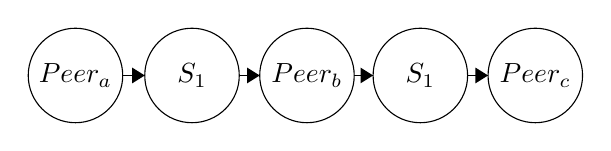
\begin{tikzpicture}[scale=0.2]
      \tikzstyle{every node}+=[inner sep=0pt]
      \draw [black] (15.3,-22.1) circle (3);
      \draw (15.3,-22.1) node {$Peer_a$};
      \draw [black] (22.7,-22.1) circle (3);
      \draw (22.7,-22.1) node {$S_1$};
      \draw [black] (30,-22.1) circle (3);
      \draw (30,-22.1) node {$Peer_b$};
      \draw [black] (37.2,-22.1) circle (3);
      \draw (37.2,-22.1) node {$S_1$};
      \draw [black] (44.5,-22.1) circle (3);
      \draw (44.5,-22.1) node {$Peer_c$};
      \draw [black] (18.3,-22.1) -- (19.7,-22.1);
      \fill [black] (19.7,-22.1) -- (18.9,-21.6) -- (18.9,-22.6);
      \draw [black] (25.7,-22.1) -- (27,-22.1);
      \fill [black] (27,-22.1) -- (26.2,-21.6) -- (26.2,-22.6);
      \draw [black] (33,-22.1) -- (34.2,-22.1);
      \fill [black] (34.2,-22.1) -- (33.4,-21.6) -- (33.4,-22.6);
      \draw [black] (40.2,-22.1) -- (41.5,-22.1);
      \fill [black] (41.5,-22.1) -- (40.7,-21.6) -- (40.7,-22.6);
    \end{tikzpicture}
  \end{center}
  \caption{A simple pseudo-P2P circuit}
\end{figure}


\subsection{Basic Protocol}
\label{sec:basic}
Assume that Alice has obtained Bob's public key and unique ID while maintaining her anonymity. This could be achieved using our directory service as outlined in Section~\ref{sec:PIRDirectories}, or by exchanging keys in advance through some other channel. Assume also that Alice can obtain the public keys and IDs for $n \le N$ peers at random while hiding her choice from Surge (This again can be done using the service in Section~\ref{sec:PIRDirectories}).

Alice can then send a message to Bob that will follow the path 
\\$A \rightarrow P_1 \rightarrow S \rightarrow P_2 \rightarrow ... \rightarrow S \rightarrow P_n \rightarrow S \rightarrow B$ 
She sends this message by wrapping the initial data in successive layers of message headers and encryption as in Figure~\ref{messageStructure}.
\\
\begin{figure}[h]
Let \scriptsize$M = ID_A||E_{KRA}[ header || time || nonce || message ]$
\normalsize
\\Let \scriptsize$F_{ij}[x] = header||E_{KUi}[ ID_j || E_{KUj}[ x ] ]$
\normalsize
\\
Final Message: $F_{S1}[F_{S2}[...F_{SB}[ M ]]]$
\caption{Message Structure}
\label{messageStructure}
\end{figure}

Each successive party receives a message and an ID to forward that message to, and only that party can read its message. Any Penguin or Proletariat without collusion from Surge doesn't gain any information about the source or destination of the message it's passing along. 

Note that Surge can't track a message by its contents, since it gets decrypted and changed by each successive peer. 

In this system, peers operate exactly as Mixes in the literature \cite{chaum-mix} . That is, they prevent traffic correlation by removing a layer of encryption, as well (as we will discuss) by reordering and batching messages. 

This system is designed so that without collusion from Surge, Penguins or a Proletariat are powerless to do anything but to delay or fail to forward messages. They don't know the ID of the next person they are forwarding the message to (since it's encrypted with the server's key), and obtain no other information when forwarding messages. 
\subsection{Security Flaws}
Here we will perform a simplified analysis of the security flaws of the basic, na\"ive system described so far. 
Let $P_{AB}$ be the probability that Alice sent a given message that was delivered to to Bob. 
\begin{enumerate}
\item\textbf{Linear Chain.} If we assume that Alice's message is the only message sent by any of $p_1 \ldots p_n$ where $p_i$ is a peer, Surge can determine that $P_{AB} > (n+1)^{-1} \gg 1/N$. This is because Surge knows that one of $A \cup \{p_1 \ldots p_n\}$ talked to Bob.
\item\textbf{Collusion.} If $s$ peers collude with Surge to form The Fort, then The Fort can determine on average (depending on which peers Alice picked), that $P_{AB} > (n/(N-s)+1)^{-1}$ - that is, Alice has a chance $1 - (N-s)/N$ of each peer being compromised and not contributing to her privacy.
\item\textbf{Timing.} Even if $p_1 ... p_n$ are sending other messages, if Surge knows the probability distribution of the peer delay between receiving a message and forwarding it, he can discover the increased probability that Alice and Bob are talking. 
\item\textbf{Multiple Communications.} If Alice sends another message to Bob, or Bob back to Alice, the chance that they are communicating increases dramatically. 
\item\textbf{Man in the Middle.} If Alice acquries Bob's public key from Surge (and vice-versa), there's nothing to stop Surge from mounting a Man in the Middle attack given this simple model. 
\end{enumerate}
This is fairly poor security. If Alice chooses $n = 5$, then if her chosen peers send no other messages until hers is delivered, Surge knows $P_{AB}$, the probability that Alice is talking to Bob, is $> 1/6$. If $60\%$ of peers are part of the Fort, then Surge possibly knows $P_{AB} = 1$ (if $n \subset s$), but the expectation is $E[P_{AB}] = 1/3$ which is very poor anonymity.

\section{Improved Protocol}
To begin solving these problems, we will need to change the protocol so that any non-Penguin peer will always wait until it can send \textbf{two or more messages simultaneously}. This is equivilant to turning each peer into a 2-threshold mix. \cite{trickle02}

If we assume that The Fort has not been established (no peers are colluding with Surge), then Alice only needs to choose $n = \log(N)$ to remain anonymous from Surge. If every node sends 2 messages at once, and her message passes through $\log(N)$ nodes, then there are $2^n = 2^{\log(n)} = N$ possible messages that Alice sent, and some $< N$ possible destinations. The likelihood is that in $\log(N)$ steps from Alice, there will be less than $2^n = N$ unique recipients of messages, but we can adjust for this by increasing the number of nodes $n$ we choose. If every node has an average unique branching factor of $z$ rather than $2$, we can just set $n = \log_z(N)$ and then $z^{\log_z(N)} = N$. Then, the size of Alice's anonymity probability distribution is $\approx 1$ since the sender probabilities are roughly uniform.

In this way Surge gains no information about the sender of the message. If Surge knows Alice will choose $n = \log(N)$, then he can rule out any peer in the chain with distance less than $n$ from Alice, and then $P_{AB} = 2^{-(\log(N)-1)} = 2/N$, and $S = - \frac{1}{4} \log(\frac{1}{2N})$ which is still reasonable, though Alice could compensate further by randomly choosing the length of her circuit. 


\subsection{Peers as Mixes}
\label{sec:PeersAsMixes}
As previously discussed, peers act as mixes in this system - inheriting both their benefits and vulnerabilities. Many types of mixes have been developed, and Serjantov \cite{trickle02} has compiled common attacks and solutions. 
A mix holds on to incoming messages until its \textbf{flush function} is satisfied, then it forwards some subset of its collected messages. Common attacks are variants of the $n - 1$, or $flooding$ attack, in which an attacker fills the mix with its own fake messages and then sends the 1 message he wishes to track. 

All known mix types are vulnerable to such exact attacks \cite{trickle02} -  attacks that allow an attacker to know whether his attack was successful or not and try again if not. Since in our threat model Surge has complete access to the message history of each peer as well as the ability to delay and insert as many messages as he desires, trying to prevent these attacks by implementing a better flush function is even more futile. 

In our case, Surge can bypass the benefits obtained from turning peers into 2-Threshhold mixes by delivering one of his own false message-forward-requests along with every real message sent to each peer, so he can disregard one branch and essentially remove the anonymity gained from each hop in the circuit. 

Fortunately, due to the nature of this system we can provide almost complete protection with \textbf{cover traffic} \cite{trickle02}, or having each peer send dummy messages along with the messages it's forwarding. A peer will at minimum send one dummy message along with every real message, maintaining a branching factor greater than two at every hop. Typically, obtaining complete protection with cover traffic is difficult - it requires the mix to choose dummy message recipients uniformally from all users\cite{trickle02}. In our system, however, randomly and anonymously choosing other online peers is designed to be efficient.

It would also be possible to use inter-mix detours\cite{trickle02}, having peers randomly decide to introduce new hops to prevent Surge from recognizing his own messages sent during an $n - 1$ attack. However, this reduces reliability, increases latency, and given the protection that cover traffic provides seems unnecessary in this system. 

 In mix systems, it is important that messages are padded to be the same length to prevent message correlation \cite{chaum-mix}. Without this, Surge can inspect the size of messages sent to a peer and gain information about which incoming messages might be outgoing messages. 

\subsection{Anonymity inside The Fort} 
\label{sec:thefort}
Using this improved pseudo-P2P message system, we will analyze the security of Alice sending a single message to Bob when Surge colludes with Penguins to form The Fort. 

Assuming the set $S$ of peers colludes with the server where $s = |S| > n$, and Alice chooses her circuit $C$ of peers randomly (where $|C| = n$), there is some chance that all chosen peers are colluding with Surge $(R \subset S)$ and so Alice's identity is completely compromised $(P_{AB} = 1$ and $S = 0)$. 

Let $\phi$ be the proportion of peers who are colluding with Surge. Then $s = \phi N$ peers are part of The Fort, and on average $(1 - \phi)n$ of $n$ chosen peers still help maintain privacy, leading to the expectation $E[P_{AB}] = 2^{-(1 - \phi) \log(N)}$. 

The chance Surge can tell with probability greater than $\gamma$ that Alice and Bob are talking to each other, $p(P_{AB} > \gamma)$, gives reasonable intuition into the \textit{worst-case} security of the system considering passing messages through circuits of peers. It can be interpreted as the probability that Alice has been ``found out'' to some specified degree. 

If we assume that Alice is the ``prime suspect'', and that all other peers have a uniform distribution of probability assigned to them, we get that $S$ (the number of bits the attacker still needs to gain) is:

\begin{center}
$-S = (1 - \gamma) \log(\frac{1-\gamma}{N - 1}) + \gamma \log(\gamma)$
\end{center}

To gain an intuition about what values of $\gamma$ mean, we can then plot $S$ for various values of $\gamma$
\begin{figure}[h!]
  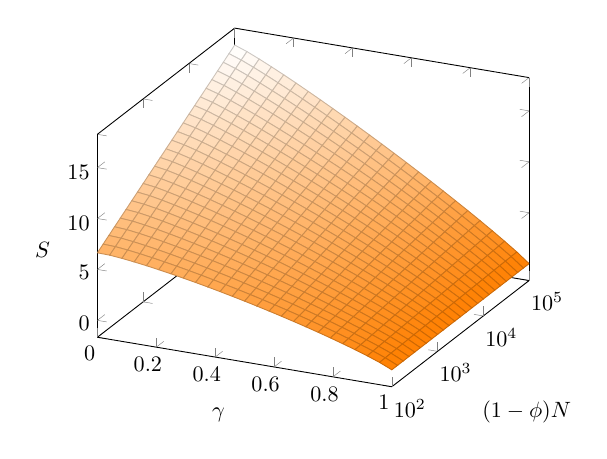
\begin{tikzpicture}[scale=0.8]
    \begin{axis}[
      xlabel=$\gamma$
      ,ylabel = $(1-\phi)N$
      ,zlabel = $S$
      ,z label style = {rotate=270}
      ,ztick = {0,5,...,25}
      ,ytick = {100, 1000, 10000, 100000}
      ,ymode = log
      ,log basis y={10}
      ]
      \addplot3[surf, mesh/interior colormap={blueblack}{color=(orange) color=(white)},
      colormap/blackwhite, domain=0:1, y domain =100:100000, range = 0:20] { -1 * (((1 - x) * log2((1 - x)/(y-1)) + x * log2(x) )) };
    \end{axis}
  \end{tikzpicture}  
  \caption{Relating $\gamma$ and $S$}
  \label{gammaS}
\end{figure}

As we can see in Figure~\ref{gammaS}, having additional peers in the network (higher $N$ values) only helps increase Alice's anonymity ($S$ value) when $\gamma$ is small. That is, having more peers in the network doesn't really mitigate the security lost if Surge already believes that Alice sent a message with probability $0 \ll \gamma < 1 $. 

\subsection{Likelihood of the worst-case}
\label{sec:worstcase}
We'd like to know how likely the worst-case ($p(P_{AB} > \gamma)$) scenario is given the circuit length chosen by Alice. 

If we let $x$ be the number of compromised peers Alice must choose such that $p(P_{AB} > \gamma)$, we obtain: 
\begin{center}
$\gamma = P_{AB} = 2^{-(n - x)} = 2^{-(\log(N) - x)}$
\\ $ \Rightarrow x = log( \gamma ) + n$
\end{center}
Each peer has a probability $\phi$ of being part of the Fort, so Alice choosing $x$ or more colluding peers occurs with probability:
\begin{center}
 $p(P_{AB} > \gamma) = \mathlarger{\sum}\limits_{i=\log(\gamma) + n}^n {n \choose i} \phi^i (1 - \phi )^{n-i}$

\end{center}

Intuitively, Alice would be in an anonymity set of size 2 when $\gamma = 0.5$. This happens when all but one nodes are compromised, as indicated by our derived value $x = log( 0.5 ) + n = n - 1$. 

\begin{figure}[h]
  \small
  \begin{tabular}{| l | l | l | l | l | l |}

    \hline
    $\phi$ & N & n & x & $E[P_{AB}]$ & $p(P_{AB} > 0.5)$ \\\hline
    0.8 & 1000 & 10 & 9 & 0.031 & 0.38\\
    0.8 & 10000 & 14 & 13 & 0.010 & 0.20\\
    0.8 & 100000 & 17 & 16 & 0.003 & 0.12\\
    \hline
  \end{tabular}
  \caption{Probability of the worst-case}
  \label{WorstCaseTable}
\end{figure}

As seen in Table~\ref{WorstCaseTable} , the chance that Surge, having $80\%$ of 10000 peers colluding with him, can tell that Alice is talking to Bob with probability greater than $0.5$ is $20\%$. For reference, if Surge believes $P_{AB} = 0.5$ given the 2000 uncompromised peers, then the probability distribution size $S = 1.93$. 

\subsection{Longer Circuits}
If this level of security is unacceptable, the length of the circuit can be chosen based on an estimate of $\phi$ and an acceptable $p(P_{AB} > \gamma)$. Assuming $\gamma = 0.5$, then 
\begin{center}
$p(P_{AB} > 0.5)$ = $n\phi^{n-1} (1 - \phi ) + \phi^n $
\end{center}

Although n is difficult to solve for directly (requiring the Lambert W equation), a we give a graph for $n$ and $\phi$ given $\gamma = 0.5$:

\begin{figure}[h]
\includegraphics*[width=\linewidth]{gamma5graph.eps}
\caption{$p(P_{AB} > 0.5)$ given $n$ and $\phi$}
\label{gamma5graph}
\end{figure}

Given Figure~\ref{gamma5graph} it's clear that if the network is believed to be widely compromised, security can be made up for by choosing longer circuits. Although $\phi = 0.8$ makes $n = 10$ an unviable choice, at a circuit length of $n=20$ having $\phi = 0.8$ barely increases the likelihood of the worst-case. 

\begin{comment}
  TODO: Apply PIR to obtain security guarantees even when $R \subset S$
\end{comment}

\section{Peer Information Retrieval}
Our system stores all information about which peers are online and their public keys in the central server. 

If Alice wishes to send a message to Bob, she needs to obtain the ID and public key for $n$ peers from the central server, as well as Bob's public key. To perform this request securely and efficiently, we use Private Information Retrieval (PIR).


\subsection{Private Information Retrieval}
  If Alice queried for information about these peers using a typical database, Surge would gain information about both who she is possibly talking to and which peers she uses in her circuits, dramatically reducing Alice's anonymity. 

However, using Private Information Retrieval, it is possible to have Alice obtain this information without the server getting any information about the records she retrieved. 

As a proof of concept, our system implements Gentry's CPIR system \cite{singledatabaseprivate}, which uses cyclic groups of prime powers to encode requests for data, and performs group operations to create a database response. This system has been analyzed and found to be less efficient than sending the entire database \cite{practicalPIR}(when considering a combination of both computation and communication overhead), but in the future we will implement a much faster lattice based system as analyzed by Olumofin and Goldberg in \cite{practicalPIR}.

\subsection{Using PIR For Directories}
\label{sec:PIRDirectories}
To allow Alice to get information about which peers are online, their public keys, and the public keys of people she wishes to communicate with, we maintain two PIR databases.

The first is a database of peers currently online (Figure~\ref{onlinePeerDB}), indexable by an integer between 0 and $N$, the number of online peers. To reduce the number of PIR requests, we redundantly include the public keys in this database. Alice chooses peers for her circuits by querying using random indexes in this database:

\begin{figure}[ht]
  \centering
\begin{tabular}{| l | l | l |}
  \hline
  Record ID & Peer ID & Peer Public Key \\ \hline
  0 & 687542 & $pubkey_{687542}$  \\ \hline
  1 & 552455 & $pubkey_{552455}$  \\ \hline
  ... & ... & $...$  \\ \hline
  $N$ & 432314 & $pubkey_{432314}$  \\ \hline
\end{tabular}
\caption{The Online-Peer Database}
\label{onlinePeerDB}
\end{figure}

The second is a similar database (Figure~\ref{peerKeyDB}), that contains all known peers (online and offline) and is indexable by a user's ID. Alice uses this database to lookup the public keys of message recipients by their peer ID (which she can't do in the first database). 

\begin{figure}[ht]
  \centering
\begin{tabular}{| l | l | }
  \hline
  Peer ID & Peer Public Key  \\ \hline
  909787 & $pubkey_{909787}$ \\ \hline
  424566 & $pubkey_{424566}$ \\ \hline
  ... & ... \\ \hline
  432314 & $pubkey_{432314}$  \\ \hline
\end{tabular}
\caption{The Peer Key Database}
\label{peerKeyDB}
\end{figure}

\subsection{Peer Discovery}
\label{sec:PeerDiscovery}
Using the model described above, choosing random peers for use in a circuit is efficient for users.  Unfortunately, if peers discover eachother through Surge, he could ensure that any peer only knows about compromised peers (Effectively making $\phi = 1$).

This is a common problem in Onion routing schemes like Tor, as well as Mix networks. If directory servers collude with some routing servers, they can choose to only broadcast the existence of the compromised routing servers.

MixMinion \cite{minion-design} solves these problems by having a small group of directory servers that only update nightly, having servers sign each other's directories, and ensuring that users download entire directories. This solution is not feasible because set of online users is constantly changing. Sending the entire user list to every user each time someone logs on or off is infeasable. Tor \cite{tor-design} likewise has a small number of trusted directory servers that share infrequently updated, signed directories.

In our system, however, a compromised Surge is disincentivized from lying about which peers are online. Consider a situation in which Alice wishes to send a message to Bob. If Surge doesn't report any non-colluding peers as online, then Alice won't send any messages to Bob since he appears to be offline. If Surge doesn't exclude non-colluding peers from the online list, however, Alice will inevitably include some of them in her chosen circuits. Since Surge doesn't know that Alice and Bob are communicating beforehand, he is forced to either include or exclude all non-colluding peers from the online-peers database~as~a~whole. 


\subsection{Man in the Middle} 

In this model, it's trivial for Surge to mount a Man in the Middle attack. If Alice wishes to talk to Bob, she first obtains Bob's public key from Surge. If Surge lies about Bob's public key to everyone but Bob, he can intercept all messages sent to Bob, decrypt them with a fake private key he generated for Bob, and re-encrypt them with Bob's real public key. In this way no one realizes that all of Bob's messages are being intercepted. 

 Assuming that Surge can't lie about real peers being online (as discussed in Section~\ref{sec:PeerDiscovery}), Bob simply needs to ask random peers to query Surge for Bob's public key and send him the result (We will call this \textbf{Auditing}). Requests sent to peers colluding with Surge could be faked, but Bob can send enough requests to gain any level of confidence he wishes that his key is being correctly distributed. 

If Surge is willing to allow Bob to learn that he's lying about public keys, Surge can share a fake public key with the world and masquerade as Bob, intercepting all initial messages sent to him and potentially learning the identities of Bob's associates. Worse, he could masquerade as Bob when he knows Bob is offline.

The solution to this attack is twofold: users need to store the keys of friends and acquaintances they trust, and the protocol should ensure that initial communications don't include uniquely identifying information about the sender (perhaps using pseudonymous communication for the initial request).

\subsection{Trust}

Man in the Middle attacks can be further mitigated by maintaining a web of trust of public keys. To obtain an initial web of trust, we will use the PGP web of trust \cite{zimmermann1995official} in this system. Users may import their PGP keys and use them as their public keys on the system. This may tie user identities in the system to real identities, but this could be avoided by implementing pseudonymity in the system, and by allowing users to elect to use new keys. 




\section{Future Work}
\begin{description}
\item[Pseudonymity and offline message delivery.] We would like to allow for parties to communicate securely without knowing each other's identities. Currently our system relies heavily on a peer knowing the public key of the final recipient of their message. 

To obtain both pseudonymity and offline message delivery, we could employ a Pynchon Gate as developed by Sassaman \cite{sassaman:wpes2005}. We would need to use CPIR instead of ITPIR since we are employing a single central server, but the same principle allowing for pseudonymity applies. 

\item[Faster encryption.] Like Tor, we could use layers of symmetric encryption between successive pairs of peers in a circuit. Using a public/symmetric system like Tor could help with pseudonymity as well. Currently we are doing a lot of public/private key encryption which is slow.

\item[DoS.] We would like to address the issue of DoS attacks against networks by requiring messages to be accompanied by a proof of work. This would allow us to require that the messages being sent are by computers that are also helping to suport the network.

\item[Peer Storage.]
  Ultimately it will be necessary for the system to offer storage to peers using the network. This will allow peers to store their keyring on the central server, as well as mail that they have already received. The data stored by the server would be encrypted entirely by the peer, ensuring that the server can't obtain the contents of their mail, which keys they trust, etc.  

\item[Applying PIR to Routing]
We could potentially reduce the length of circuits by using PIR databases as a hop in the chain. An obvious way to utilize PIR for anonymous communication is as a ``Dead Drop''. If we have a PIR server Charlie, Alice could write her messages to block $i$ in Charlie's PIR database, then Bob could request block $i$ anonymously. This could enable us to increase the size of Alice's anonymity set (retaining a uniform distribution of probabilities, as well) while reducing our circuit length significantly. 

There are, however, several problems with this configuration.

First, Alice must communicate Charlie's ID and $i$ to Bob anonymously. This could happen via the pseudo-P2P protocol as above. 

Second, Alice and Bob both start talking to Charlie around the same time. If Charlie suspects Alice and Bob are talking to each other, he can easily create a fake PIR database for all of Alice's inserts and all of Bob's retrievals, and if they continue to communicate normally he has discovered a connection. 

We would like to develop this strategy further in the future - at present, it is not efficient or secure enough to employ.
\end{description}

\section{Summary}
 We've summarized some of the key points of the protocol in Figure~\ref{fig:keypoints}, and give a broad outline of the protocol below:

\begin{figure*}[scale=0.7]
\includegraphics{summary.eps}
\caption{Key Points of Protocol Summary}
\label{fig:keypoints}
\end{figure*}

\begin{enumerate}
  
  \item The central server houses two Private Information Retrieval databases: one containing all online users, and one containing all user's keys. Peers can only communicate indirectly through the server, and always do so with encrypted messages. 
  \item Messages are sent using the basic structure from Section~\ref{sec:basic}, using layers of public key encryption to pass through the server and peers in an alternating fashion. 
  \item Circuits through which messages are sent are chosen by the peer who wishes to send a message. These circuits are chosen randomly from the server's PIR database of online users. The circuit length can be chosen as $log(N)$ where $N$ is the number of online users, as discussed in Section~\ref{sec:thefort}, or according to acceptable risk as discussed in Section~\ref{sec:worstcase}.
  \item Peers act as relays for other peers, but don't know the true destination of messages they decrypt and relay back to the server. It's important that since peers act as mixes (Section~\ref{sec:PeersAsMixes}), they always wait until they receive two messages before they forward them onward, that messages are always padded to a fixed length, and that peers always generate 1 fake message as cover traffic, using a circuit length of at least 1 hop.
  \item Peers need to audit their public keys by requesting that other peers request their public key and relay it back to them, to make man-in-the-middle attacks more challenging. Additionally, peers need to store the retrieved keys of other peers in order to detect discrepancies that could indicate an attack. Keys should be signed and given trust levels as in PGP to further mitigate this risk. 
\end{enumerate}

\section{Conclusion}
In this paper, we have introduced a system for sending anonymous messages via a central server with low-latency. This system is designed to prevent the correlation between the sender and receiver of messages, using an adaption of P2P protocols to the central server setting. We analyzed the probabilistic security of using peers as 2-threshhold mixes given different circuit lengths.

We showed that malicious peers on their own only have the power to delay or prevent message delivery. When colluding with the central server, peers can only reduce a sender's security probabilistically. This risk can be mitigated by circuit length. To prevent attacks by the central server using its databases and knowledge of keys, we have suggested the use of a web of trust, auditing, and key storage. 
\newpage
\begin{figure*}
\bibliography{paper.bib}
\bibliographystyle{unsrt}
\end{figure*}
\end{document}
